\documentclass[10pt,a4paper,onecolumn]{article}
\usepackage{marginnote}
\usepackage{graphicx}
\usepackage{xcolor}
\usepackage{authblk,etoolbox}
\usepackage{titlesec}
\usepackage{calc}
\usepackage{tikz}
\usepackage{hyperref}
\hypersetup{colorlinks,breaklinks,
            urlcolor=[rgb]{0.0, 0.5, 1.0},
            linkcolor=[rgb]{0.0, 0.5, 1.0}}
\usepackage{caption}
\usepackage{tcolorbox}
\usepackage{amssymb,amsmath}
\usepackage{ifxetex,ifluatex}
\usepackage{seqsplit}
\usepackage{fixltx2e} % provides \textsubscript
\usepackage[
  backend=biber,
%  style=alphabetic,
%  citestyle=numeric
]{biblatex}
\bibliography{paper.bib}



% --- Page layout -------------------------------------------------------------
\usepackage[top=3.5cm, bottom=3cm, right=1.5cm, left=1.0cm,
            headheight=2.2cm, reversemp, includemp, marginparwidth=4.5cm]{geometry}

% --- Default font ------------------------------------------------------------
% \renewcommand\familydefault{\sfdefault}

% --- Style -------------------------------------------------------------------
\renewcommand{\bibfont}{\small \sffamily}
\renewcommand{\captionfont}{\small\sffamily}
\renewcommand{\captionlabelfont}{\bfseries}

% --- Section/SubSection/SubSubSection ----------------------------------------
\titleformat{\section}
  {\normalfont\sffamily\Large\bfseries}
  {}{0pt}{}
\titleformat{\subsection}
  {\normalfont\sffamily\large\bfseries}
  {}{0pt}{}
\titleformat{\subsubsection}
  {\normalfont\sffamily\bfseries}
  {}{0pt}{}
\titleformat*{\paragraph}
  {\sffamily\normalsize}


% --- Header / Footer ---------------------------------------------------------
\usepackage{fancyhdr}
\pagestyle{fancy}
\fancyhf{}
%\renewcommand{\headrulewidth}{0.50pt}
\renewcommand{\headrulewidth}{0pt}
\fancyhead[L]{\hspace{-0.75cm}\includegraphics[width=5.5cm]{/Library/Frameworks/R.framework/Versions/4.4-arm64/Resources/library/rticles/rmarkdown/templates/joss/resources/JOSS-logo.png}}
\fancyhead[C]{}
\fancyhead[R]{}
\renewcommand{\footrulewidth}{0.25pt}

\fancyfoot[L]{\footnotesize{\sffamily Jayaprakash et al., (2024). Nemo
Gradebook: An R Package for Calculating Course
Grades. \textit{Journal of Open Source Software}, (), . \href{https://doi.org/}{https://doi.org/}}}


\fancyfoot[R]{\sffamily \thepage}
\makeatletter
\let\ps@plain\ps@fancy
\fancyheadoffset[L]{4.5cm}
\fancyfootoffset[L]{4.5cm}

% --- Macros ---------

\definecolor{linky}{rgb}{0.0, 0.5, 1.0}

\newtcolorbox{repobox}
   {colback=red, colframe=red!75!black,
     boxrule=0.5pt, arc=2pt, left=6pt, right=6pt, top=3pt, bottom=3pt}

\newcommand{\ExternalLink}{%
   \tikz[x=1.2ex, y=1.2ex, baseline=-0.05ex]{%
       \begin{scope}[x=1ex, y=1ex]
           \clip (-0.1,-0.1)
               --++ (-0, 1.2)
               --++ (0.6, 0)
               --++ (0, -0.6)
               --++ (0.6, 0)
               --++ (0, -1);
           \path[draw,
               line width = 0.5,
               rounded corners=0.5]
               (0,0) rectangle (1,1);
       \end{scope}
       \path[draw, line width = 0.5] (0.5, 0.5)
           -- (1, 1);
       \path[draw, line width = 0.5] (0.6, 1)
           -- (1, 1) -- (1, 0.6);
       }
   }

% --- Title / Authors ---------------------------------------------------------
% patch \maketitle so that it doesn't center
\patchcmd{\@maketitle}{center}{flushleft}{}{}
\patchcmd{\@maketitle}{center}{flushleft}{}{}
% patch \maketitle so that the font size for the title is normal
\patchcmd{\@maketitle}{\LARGE}{\LARGE\sffamily}{}{}
% patch the patch by authblk so that the author block is flush left
\def\maketitle{{%
  \renewenvironment{tabular}[2][]
    {\begin{flushleft}}
    {\end{flushleft}}
  \AB@maketitle}}
\makeatletter
\renewcommand\AB@affilsepx{ \protect\Affilfont}
%\renewcommand\AB@affilnote[1]{{\bfseries #1}\hspace{2pt}}
\renewcommand\AB@affilnote[1]{{\bfseries #1}\hspace{3pt}}
\makeatother
\renewcommand\Authfont{\sffamily\bfseries}
\renewcommand\Affilfont{\sffamily\small\mdseries}
\setlength{\affilsep}{1em}


\ifnum 0\ifxetex 1\fi\ifluatex 1\fi=0 % if pdftex
  \usepackage[T1]{fontenc}
  \usepackage[utf8]{inputenc}

\else % if luatex or xelatex
  \ifxetex
    \usepackage{mathspec}
  \else
    \usepackage{fontspec}
  \fi
  \defaultfontfeatures{Ligatures=TeX,Scale=MatchLowercase}

\fi
% use upquote if available, for straight quotes in verbatim environments
\IfFileExists{upquote.sty}{\usepackage{upquote}}{}
% use microtype if available
\IfFileExists{microtype.sty}{%
\usepackage{microtype}
\UseMicrotypeSet[protrusion]{basicmath} % disable protrusion for tt fonts
}{}

\usepackage{hyperref}
\hypersetup{unicode=true,
            pdftitle={Nemo Gradebook: An R Package for Calculating Course Grades},
            pdfborder={0 0 0},
            breaklinks=true}
\urlstyle{same}  % don't use monospace font for urls
\usepackage{graphicx,grffile}
\makeatletter
\def\maxwidth{\ifdim\Gin@nat@width>\linewidth\linewidth\else\Gin@nat@width\fi}
\def\maxheight{\ifdim\Gin@nat@height>\textheight\textheight\else\Gin@nat@height\fi}
\makeatother
% Scale images if necessary, so that they will not overflow the page
% margins by default, and it is still possible to overwrite the defaults
% using explicit options in \includegraphics[width, height, ...]{}
\setkeys{Gin}{width=\maxwidth,height=\maxheight,keepaspectratio}
\IfFileExists{parskip.sty}{%
\usepackage{parskip}
}{% else
\setlength{\parindent}{0pt}
\setlength{\parskip}{6pt plus 2pt minus 1pt}
}
\setlength{\emergencystretch}{3em}  % prevent overfull lines
\setcounter{secnumdepth}{0}
% Redefines (sub)paragraphs to behave more like sections
\ifx\paragraph\undefined\else
\let\oldparagraph\paragraph
\renewcommand{\paragraph}[1]{\oldparagraph{#1}\mbox{}}
\fi
\ifx\subparagraph\undefined\else
\let\oldsubparagraph\subparagraph
\renewcommand{\subparagraph}[1]{\oldsubparagraph{#1}\mbox{}}
\fi


% tightlist command for lists without linebreak
\providecommand{\tightlist}{%
  \setlength{\itemsep}{0pt}\setlength{\parskip}{0pt}}

% From pandoc table feature
\usepackage{longtable,booktabs,array}
\usepackage{calc} % for calculating minipage widths
% Correct order of tables after \paragraph or \subparagraph
\usepackage{etoolbox}
\makeatletter
\patchcmd\longtable{\par}{\if@noskipsec\mbox{}\fi\par}{}{}
\makeatother
% Allow footnotes in longtable head/foot
\IfFileExists{footnotehyper.sty}{\usepackage{footnotehyper}}{\usepackage{footnote}}
\makesavenoteenv{longtable}

% Pandoc citation processing
%From Pandoc 3.1.8
% definitions for citeproc citations
\NewDocumentCommand\citeproctext{}{}
\NewDocumentCommand\citeproc{mm}{%
  \begingroup\def\citeproctext{#2}\cite{#1}\endgroup}
\makeatletter
 % allow citations to break across lines
 \let\@cite@ofmt\@firstofone
 % avoid brackets around text for \cite:
 \def\@biblabel#1{}
 \def\@cite#1#2{{#1\if@tempswa , #2\fi}}
\makeatother
\newlength{\cslhangindent}
\setlength{\cslhangindent}{1.5em}
\newlength{\csllabelwidth}
\setlength{\csllabelwidth}{3em}
\newenvironment{CSLReferences}[2] % #1 hanging-indent, #2 entry-spacing
 {\begin{list}{}{%
  \setlength{\itemindent}{0pt}
  \setlength{\leftmargin}{0pt}
  \setlength{\parsep}{0pt}
  % turn on hanging indent if param 1 is 1
  \ifodd #1
   \setlength{\leftmargin}{\cslhangindent}
   \setlength{\itemindent}{-1\cslhangindent}
  \fi
  % set entry spacing
  \setlength{\itemsep}{#2\baselineskip}}}
 {\end{list}}
\usepackage{calc}
\newcommand{\CSLBlock}[1]{#1\hfill\break}
\newcommand{\CSLLeftMargin}[1]{\parbox[t]{\csllabelwidth}{#1}}
\newcommand{\CSLRightInline}[1]{\parbox[t]{\linewidth - \csllabelwidth}{#1}\break}
\newcommand{\CSLIndent}[1]{\hspace{\cslhangindent}#1}


\newenvironment{cols}[1][]{}{}

\newenvironment{col}[1]{\begin{minipage}{#1}\ignorespaces}{%
\end{minipage}
\ifhmode\unskip\fi
\aftergroup\useignorespacesandallpars}

\def\useignorespacesandallpars#1\ignorespaces\fi{%
#1\fi\ignorespacesandallpars}

\makeatletter
\def\ignorespacesandallpars{%
  \@ifnextchar\par
    {\expandafter\ignorespacesandallpars\@gobble}%
    {}%
}
\makeatother

\title{Nemo Gradebook: An R Package for Calculating Course Grades}

        \author[1]{Nikita Jayaprakash}
          \author[1, 2]{Monika Voutov}
          \author[1]{Andrew Bray}
    
      \affil[1]{UC Berkeley, Department of Statistics}
      \affil[2]{UC Berkeley, College of Engineering}
  \date{\vspace{-5ex}}

\begin{document}
\maketitle

\marginpar{
  %\hrule
  \sffamily\small

  {\bfseries DOI:} \href{https://doi.org/}{\color{linky}{}}

  \vspace{2mm}

  {\bfseries Software}
  \begin{itemize}
    \setlength\itemsep{0em}
    \item \href{}{\color{linky}{Review}} \ExternalLink
    \item \href{}{\color{linky}{Repository}} \ExternalLink
    \item \href{}{\color{linky}{Archive}} \ExternalLink
  \end{itemize}

  \vspace{2mm}

  {\bfseries Submitted:} \\
  {\bfseries Published:} 

  \vspace{2mm}
  {\bfseries License}\\
  Authors of papers retain copyright and release the work under a Creative Commons Attribution 4.0 International License (\href{http://creativecommons.org/licenses/by/4.0/}{\color{linky}{CC-BY}}).
}

\section{Summary}\label{summary}

\texttt{Gradebook} allows for accurate and systematic computations of
the final course letter grades. These computations require two inputs: a
specifically structured YAML file representing the grading policy from
the class syllabus and the assignment grades in CSV (comma-separated
value) format from Gradescope (Singh et al. 2017) or other similar
learning management systems. The package uses these two inputs to break
down any complex syllabi into methodical computations that can be
documented and tested.

\section{Statement of Need}\label{statement-of-need}

While the final grade at the end of a course is an elementary part of
most college courses, the computations for these grades quickly become
deceptively intricate, especially with larger STEM classes that use
various complexities to accommodate a diverse student body. Even though
most classes use slight variations of the same policies, many LMS cannot
sustain these complex computations. In response, courses will turn to
hard-coded scripts. These scripts quickly accumulate hundreds of lines
of code, and there is no method to assess accuracy of the final
computation.

\texttt{Gradebook} is an R package that maintains the structure and
complexity of a course grade while guaranteeing accuracy through
comprehensive unit-testing. The challenges of consistency and precision
in grading systems are addressed by applying the practices of data
analysis and the principles of software development. The rigorous
unit-testing in the package minimizes computational error and reduces
the manual inputs, significantly lower the risks of typographic and
logical errors in scripts \ldots{} {[}insert reference about software
practices, testing, etc.{]}. Because of this, course grades can be
computed accurately and quickly: the accuracy allows course instructors
to have reliable grade computations, and the speed allows them to
compute grades throughout the semester in order to monitor student
progress. The structure of the package -- and the open-source nature of
it -- allows for courses to contribute functionality that is unique to
their course. This R package also functions as the backend of the NemoGB
Shiny app (Voutov*, Jayaprakash*, and Bray 2024), which lets the user
create their grading policy file in a straightforward way.

\begin{longtable}[]{@{}
  >{\centering\arraybackslash}p{(\columnwidth - 2\tabcolsep) * \real{0.5000}}
  >{\centering\arraybackslash}p{(\columnwidth - 2\tabcolsep) * \real{0.5000}}@{}}
\toprule\noalign{}
\begin{minipage}[b]{\linewidth}\centering
Grading Workflow WITH Nemo Gradebook
\end{minipage} & \begin{minipage}[b]{\linewidth}\centering
Grading Workflow WITHOUT Nemo Gradebook
\end{minipage} \\
\midrule\noalign{}
\endhead
\bottomrule\noalign{}
\endlastfoot
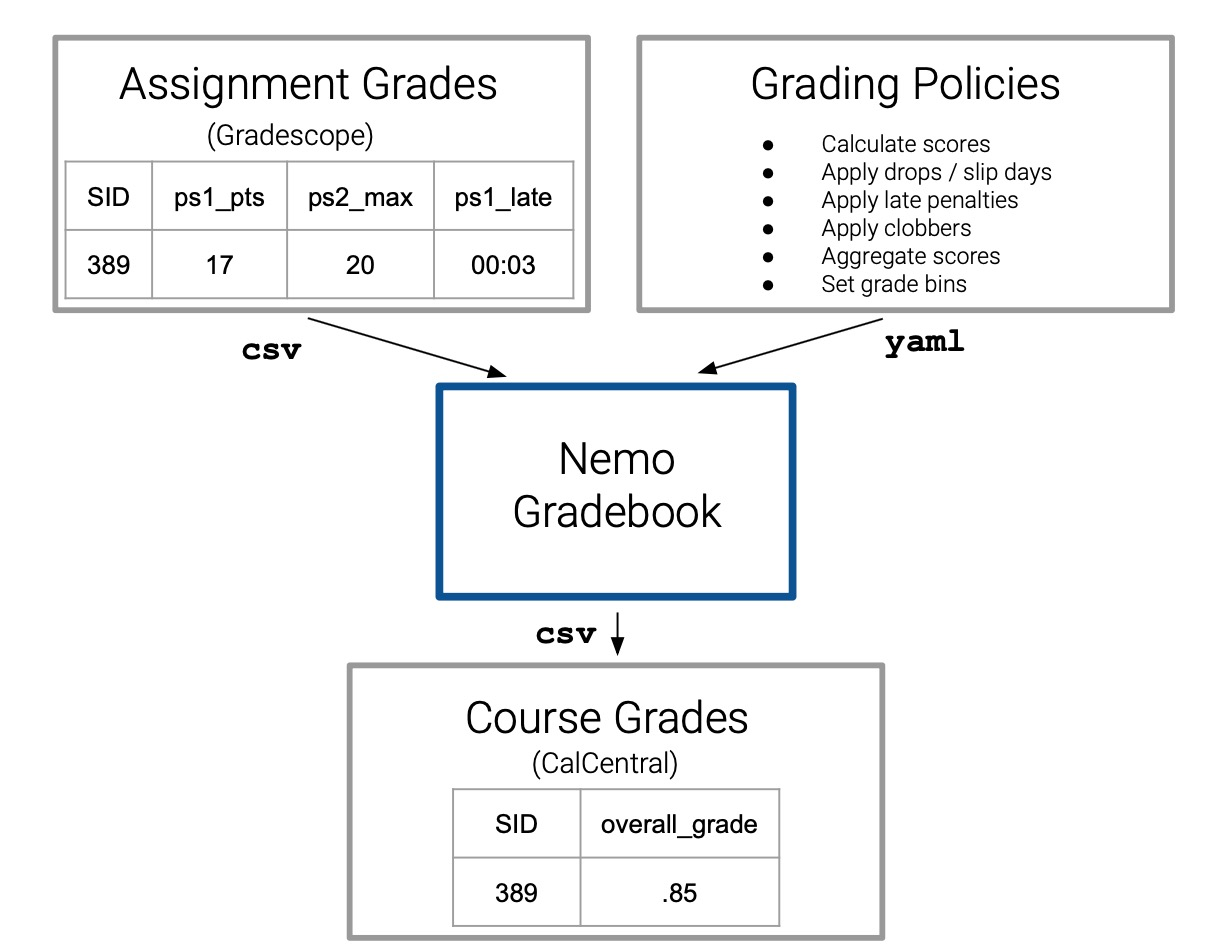
\includegraphics[width=\textwidth,height=2.08333in]{with_nemogb_workflow.png}
&
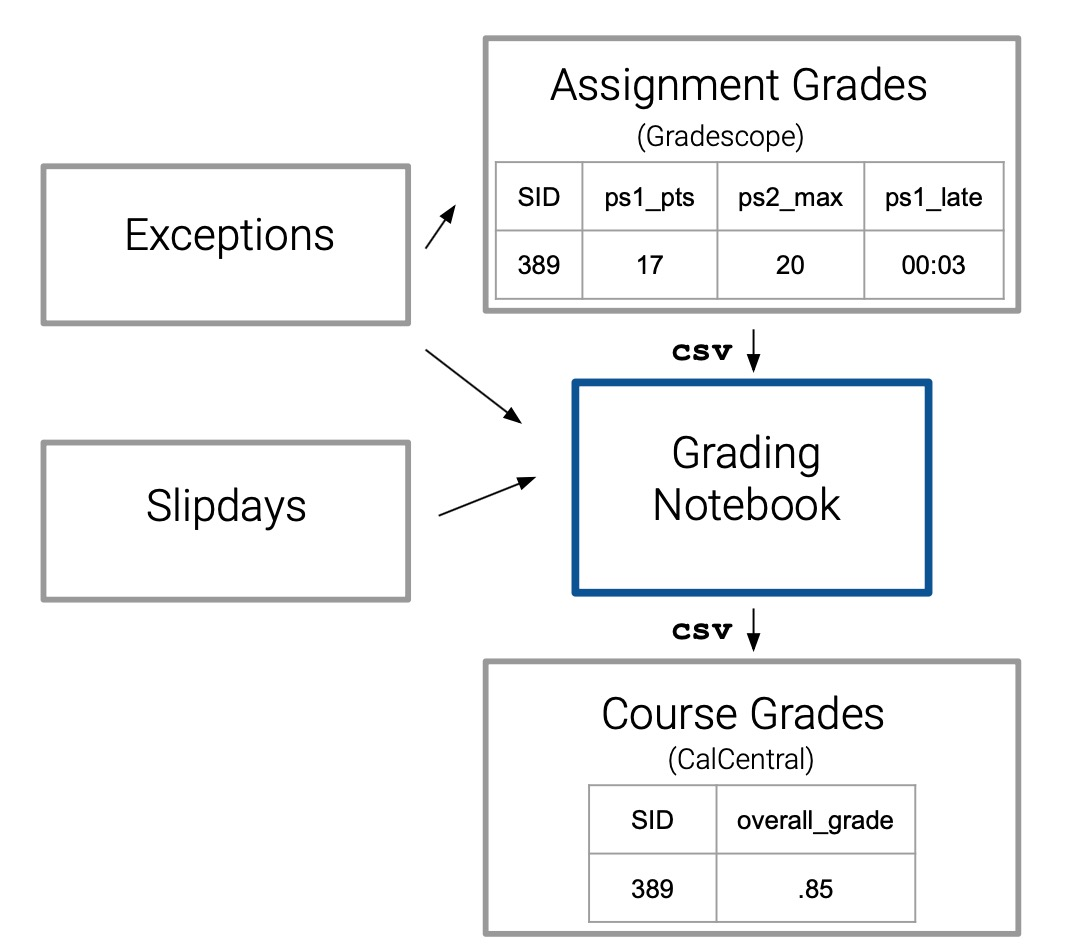
\includegraphics[width=\textwidth,height=2.08333in]{without_nemogb_workflow.png} \\
\end{longtable}

\section{Underlying Principle}\label{underlying-principle}

\texttt{Gradebook} breaks down the calculation of a course grade into a
series of nested aggregations. It accommodates the generic policies
included in most syllabi: applying lateness penalties, dropping the
\emph{n} lowest scores in a category, and using averages or weighted
averages to aggregate assignment scores into overarching category
scores. As previously mentioned, the structure of this package also
allows for outside contribution of unique policies in order for any
course structure to be computed with this package.

The details of the course grading structure -- usually detailed in the
syllabus or on the class website -- can be articulated in YAML format
using a series of accepted keys (e.g.~\texttt{score},
\texttt{aggregation}, \texttt{lateness}, \texttt{drop\_n\_lowest}, etc.)
and their corresponding inputs; more direction about creating a policy
file is provided in the \texttt{Building\ a\ Policy\ File} vignette. The
nested structure of this policy file reflects the nested structure of
the course grade. The assignment scores come directly from Gradescope in
a .csv file. These two files (the YAML policy file and the Gradescope
data) function as the two inputs for \texttt{gradebook}'s primary and
overarching function: \texttt{get\_grades()}. After reading in the
assignment data from Gradescope using \texttt{read\_gs()}and reading in
their YAML policy file (that reflects their course syllabus) using
\texttt{read\_policy()}, this singular function computes the entirety of
the final course grade computation.

While \texttt{get\_grades()} encapsulates the entire computational
functionality of the R package, it is compromised for four sequential
functions:

\begin{itemize}
\item
  \texttt{process\_gs()} ensures the correct format of the Gradescope
  csv.
\item
  \texttt{process\_policy()} similarly ensures the correct format of the
  policy file.
\item
  \texttt{reconcile\_policy\_with\_gs()} checks the compatibility of the
  policy file and the Gradescope data.
\item
  \texttt{calculate\_grades()} computes the course grades and returns
  the final grade (and the scores for every intermediate category)
  appended to the original Gradescope data.
\end{itemize}

\section{Comparison to Other
Packages}\label{comparison-to-other-packages}

Most other commonly-used packages -- particularly for R packages -- are
used for grading on an assignment-level basis. For example, the
\texttt{gradeR} package ``helps grade your students's assignment
submissions that are R Scripts'' (Brown 2021) whereas \texttt{gradebook}
is used for the computations of the final, overall course grade. The
software that has the most similar computational purpose as
\texttt{gradebook} are popular learning-management systems (LMS) used in
higher education. This includes Canvas (Canvas Community 2024), Moodle
(Moodle Docs 2024), Blackboard Learn (Blackboard Help 2024), and D2L
Brightspace (D2L Brightspace Community 2024), all of which provide an
integrated gradebook that allow the instructor to specify the manner in
which assessment scores are used to calculate a final course grade. What
makes Gradebook unique is its flexibility of functionality and its
capacity for instructor collaboration and contribution: the flexible
YAML structure allows for the former and the open-source nature of the
project allows for the latter.

\section{Acknowledgements}\label{acknowledgements}

The authors would like to thank lain Carmichael, Calvin Carter, and Zach
Turner for helpful ideas and discussions throughout the development of
this project.

As of summer 2024, we are funded by the RTL grant from the Statistics
Departmemt at University of California, Berkeley.

As of October 2024, there is a pending poster submission to Technical
Symposium on Computer Science Education (SIGCSE) that utilizes this
package, called ``Your Grades Are Wrong - Nemo Gradebook: A tool for
easy, accurate course grades''. The poster was submitted by the same set
of authors.

\section*{References}\label{references}
\addcontentsline{toc}{section}{References}

\phantomsection\label{refs}
\begin{CSLReferences}{1}{0}
\bibitem[\citeproctext]{ref-blackboard_calculate_grades}
Blackboard Help. 2024. {``Calculate Grades.''}
\url{https://help.blackboard.com/Learn/Instructor/Ultra/Grade/Grading_Tasks/Calculate_Grades}.

\bibitem[\citeproctext]{ref-GradeR}
Brown, Tylor. 2021. {``gradeR: Helps Grade Assignment Submissions That
Are r Scripts.''} \emph{GitHub Repository}.
\url{https://github.com/tbrown122387/gradeR.git}; GitHub.

\bibitem[\citeproctext]{ref-canvas_gradebook_guide}
Canvas Community. 2024. {``How Do i Use the Gradebook?''}
\url{https://community.canvaslms.com/t5/Instructor-Guide/How-do-I-use-the-Gradebook/ta-p/701}.

\bibitem[\citeproctext]{ref-d2l_about_grades}
D2L Brightspace Community. 2024. {``About Grades.''}
\url{https://community.d2l.com/brightspace/kb/articles/3305-about-grades}.

\bibitem[\citeproctext]{ref-moodle_grade_calculations}
Moodle Docs. 2024. {``Grade Calculations.''}
\url{https://docs.moodle.org/404/en/Grade_calculations}.

\bibitem[\citeproctext]{ref-10.1145ux2f3051457.3051466}
Singh, Arjun, Sergey Karayev, Kevin Gutowski, and Pieter Abbeel. 2017.
{``Gradescope: A Fast, Flexible, and Fair System for Scalable Assessment
of Handwritten Work.''} In \emph{Proceedings of the Fourth (2017) ACM
Conference on Learning @ Scale}, 81--88. L@s '17. New York, NY, USA:
Association for Computing Machinery.
\url{https://doi.org/10.1145/3051457.3051466}.

\bibitem[\citeproctext]{ref-Gradebook-App}
Voutov*, Monika, Nikita Jayaprakash*, and Andrew Bray. 2024. {``Nemo
Gradebook Web App.''} \emph{GitHub Repository}.
\url{https://github.com/gradebook-dev/gradebook-app.git}; GitHub.

\end{CSLReferences}

\end{document}
